\documentclass[12pt,a4paper]{article}

% Required Packages
\usepackage[utf8]{inputenc}
\usepackage{geometry}
\geometry{a4paper, margin=1in}
\usepackage{graphicx}
\usepackage{booktabs}
\usepackage{array}
\usepackage{hyperref}
\usepackage{float}
\usepackage{tikz}
\usetikzlibrary{shapes.geometric, arrows.meta, positioning, calc}
\usepackage{caption}
\usepackage{subcaption}
\usepackage{pgfplots} % Added for drawing real ThingSpeak graphs natively
\pgfplotsset{compat=1.18}

% TikZ Styles for Block Diagram
\tikzstyle{block} = [rectangle, draw, fill=blue!5, text width=3cm, text centered, rounded corners, minimum height=1.2cm]
\tikzstyle{mcu} = [rectangle, draw, fill=orange!5, text width=3.5cm, text centered, minimum height=3cm]
\tikzstyle{cloud} = [ellipse, draw, fill=gray!10, text width=2.5cm, text centered, minimum height=1.5cm]
\tikzstyle{line} = [draw, -Latex]

\begin{document}

% Roman numeral paging for the first sections
\pagenumbering{roman}

% Page i: Title Page
\begin{titlepage}
    \centering
    
    % Centered Logo Placeholder
    \rule{3cm}{3cm} % Replace with your actual logo, e.g., \includegraphics[width=3cm]{kyambogo_logo.png} 
    \vspace{1cm}
    
    {\Large \textbf{FACULTY OF ENGINEERING}}\\[0.2cm]
    {\large DEPARTMENT OF ELECTRICAL AND ELECTRONICS ENGINEERING}\\[0.2cm]
    {\large BACHELORS OF ENGINEERING IN TELECOMMUNICATIONS ENGINEERING}\\[0.5cm]
    
    {\large TETE/TEEE 3102: MICROCONTROLLERS}\\[1cm]
    
    \hrule
    \vspace{0.5cm}
    {\huge \textbf{LAB REPORT}}\\[0.3cm]
    {\LARGE \textbf{SMART ROOM MONITORING SYSTEM}}\\[0.2cm]
    {\Large \textbf{Level 2 Upgrade}}
    \vspace{0.5cm}
    \hrule
    \vspace{1.5cm}
    
    {\Large \textbf{Prepared By:}}
    \vspace{0.5cm}
    
    \begin{center}
        \renewcommand{\arraystretch}{1.2}
        \begin{tabular}{|c|l|c|}
            \hline
            \textbf{No.} & \textbf{Name} & \textbf{Student ID} \\
            \hline
            1 & Mukama Robert & 26/U/ETE/21285/PE \\
            2 & Nabudere Zerubabel & 25/U/ETE/05465/PE \\
            3 & Nanfuka Shakirah & 25/U/ETE/05468/PE \\
            4 & Kidega Wilkie Cephas & 25/U/ETE/05460/PE \\
            \hline
        \end{tabular}
    \end{center}
    
    \vfill
    
    \begin{flushleft}
        \textbf{Course:} TETE/TEEE 3102 \\
        \textbf{Lecturer:} Dr. Dickson Mugerwa \\
        \textbf{Group:} Group 4
    \end{flushleft}
    
    \vspace{-1.5cm}
    \begin{flushright}
        \textbf{Deadline:} 25\textsuperscript{th} August 2026 \\
        \textbf{Date Submitted:} August 31, 2026
    \end{flushright}
    
    \vspace{1cm}
    {\large \textbf{August 2026}}
\end{titlepage}

\newpage
% Page ii: Abstract
\begin{abstract}
This report details the design and implementation of the Level 2 upgrade for the Smart Room Monitoring System. Building upon the baseline parameter logging established in Level 1, this upgrade introduces complex hardware integration for enhanced security, safety, and energy profiling. An ESP32-CAM microcontroller was utilized to capture visual evidence of intrusions, while a SIM800L GSM module was integrated to ensure redundant SMS and call alerts during network outages. Additionally, ZMPT101B and ACS712 sensors were deployed to monitor AC mains voltage and current, enabling blackout detection and power consumption tracking. Telemetry and alerting are orchestrated across a robust multi-server cloud ecosystem comprising ThingSpeak, Telegram Bot API, Discord Webhook notifications, Google Colab machine-learning telemetry analytics, and a Blynk IoT mobile dashboard. The resulting prototype successfully met all functional deliverables, operating autonomously to secure and monitor the room environment.
\end{abstract}

\newpage
% Page iii: Table of Contents
\tableofcontents

\newpage
% Standard Arabic paging starting from the main content
\pagenumbering{arabic}
\setcounter{page}{1}

\section{Introduction}
The primary objective of the Level 1 Smart Room Monitoring System was to establish a basic sensor network capable of reading environmental variables and logging them to a cloud platform. While functional, it lacked the necessary countermeasures for critical events such as internet outages, power grid failures, and unverified physical intrusions.

The Level 2 upgrade addresses these limitations by shifting from a passive logging system to an active monitoring and alerting platform. The standard microcontroller was replaced with an ESP32-CAM to facilitate image capture. By expanding the sensor array to seven distinct modules—including gas detection, magnetic door switches, and AC power sensors—the system now provides a comprehensive overview of room security and grid stability. Furthermore, communication is diversified across multiple specialized cloud servers: Telegram for interactive photo alerts and remote command execution, Discord for centralized operational channel logging, Google Colab for predictive telemetry analytics, and Blynk for mobile widget control.

\section{System Objectives}
The core objectives required to fulfill the Level 2 system specifications are outlined as follows:
\begin{enumerate}
    \item \textbf{Identify:} To identify and select the necessary hardware components (such as the ESP32-CAM, SIM800L, and advanced power/gas sensors) required to upgrade the system's capabilities.
    \item \textbf{Design:} To design an integrated and robust system architecture that securely interfaces visual evidence capture, offline GSM redundancy, and real-time grid monitoring.
    \item \textbf{Deploy and Test:} To deploy the physical prototype and thoroughly test the multi-server cloud ecosystem, specifically the web dashboard (ThingSpeak), Telegram Bot API, Discord Webhooks, Google Colab data science pipeline, and Blynk IoT mobile dashboard.
    \item \textbf{Bill:} To formulate a comprehensive Bill of Materials (BOM) and cost analysis for a scaled, 100-unit deployment.
\end{enumerate}

\section{Methodology and System Design}
The system architecture was divided into hardware interfacing, logic control, and data transmission subsystems. 

\subsection{Hardware Selection}
To achieve the upgraded functionalities, the component list was expanded. The ESP32-CAM serves as the primary processing unit, replacing the previous Arduino Uno and ESP8266 combination to provide integrated Wi-Fi and camera capabilities.

\begin{table}[H]
\centering
\caption{System Hardware Components and their Functional Roles}
\label{tab:components}
\begin{tabular}{|l|p{9cm}|}
\hline
\textbf{Component} & \textbf{Function in System} \\ \hline
ESP32-CAM & Central microcontroller, image processing, and Wi-Fi interface. \\ \hline
SIM800L GSM & Secondary communication channel for SMS and voice calls. \\ \hline
ZMPT101B & AC voltage transformer for mains monitoring. \\ \hline
ACS712 (20A) & Hall-effect current sensor for power calculations. \\ \hline
MQ-2 Gas Sensor & Detects combustible gases (LPG) and smoke concentrations. \\ \hline
Magnetic Reed Switch & Physical boundary sensor for the main door or window. \\ \hline
DHT22 \& HC-SR04 & Continuous ambient temperature, humidity, and distance sampling. \\ \hline
HC-SR501 PIR & Infrared motion detection for the security logic. \\ \hline
\end{tabular}
\end{table}

\subsection{Security and Safety Logic}
The security subsystem relies on the physical state of the reed switch and the PIR sensor. When the system is armed (e.g., after 22:00 hrs) and an intrusion is detected, a hardware interrupt triggers the ESP32-CAM to capture an image. This image is immediately saved to the onboard SD card. Concurrently, the GSM module is instructed via UART to dispatch an SMS containing the time of intrusion to the administrator's mobile device.

The safety layer continuously polls the analog output of the MQ-2 sensor. If the analog reading surpasses the predefined threshold for gas or smoke, the microcontroller asserts a HIGH signal to a digital pin connected to a relay. This relay mechanically opens a window or powers an exhaust fan while activating a local buzzer.

\subsection{Power Monitoring}
To monitor the utility grid, the ZMPT101B and ACS712 sensors measure the AC voltage and current drawn by the room. The microcontroller calculates real-time power ($P = V \times I$) and integrates this over time to estimate energy consumption in kWh. If the measured voltage drops below 180V or falls to zero, a blackout condition is flagged, prompting an immediate GSM alert.

\section{System Block Diagram}
The interactions between the inputs, processing unit, and cloud interfaces are illustrated in the block diagram below.

\begin{figure}[H]
    \centering
    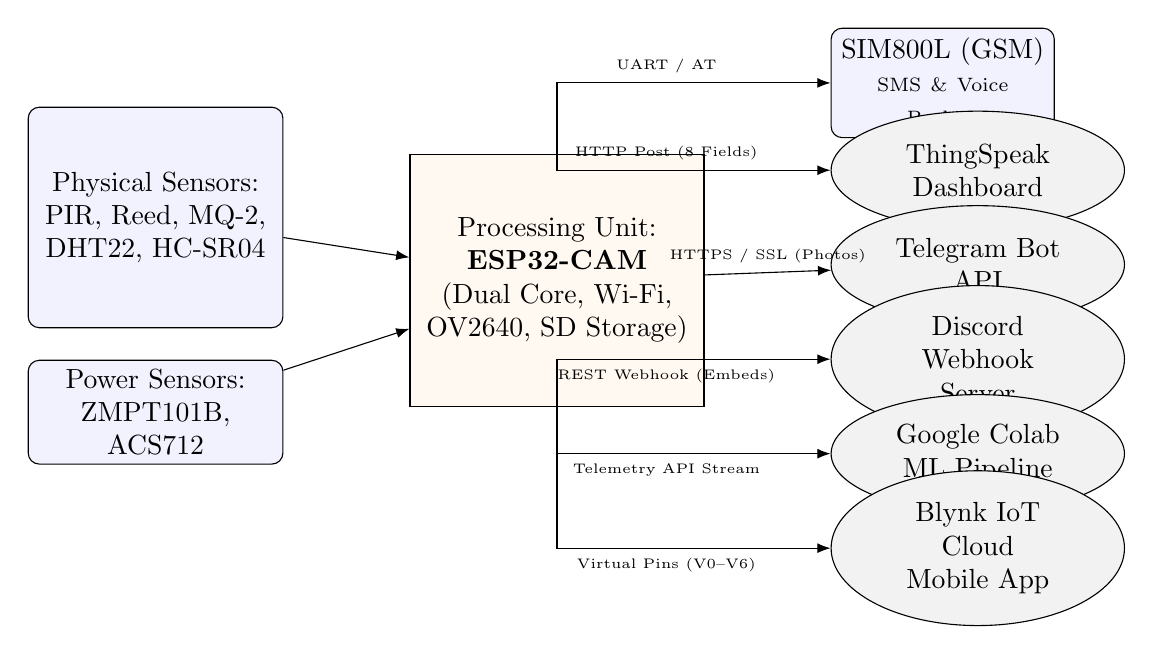
\begin{tikzpicture}[node distance=1.2cm and 1.8cm]
        
        \node (sensors) [block, minimum height=2.8cm] {Physical Sensors:\\PIR, Reed, MQ-2,\\DHT22, HC-SR04};
        \node (power) [block, below=0.4cm of sensors, minimum height=1.2cm] {Power Sensors:\\ZMPT101B, ACS712};
        
        \node (mcu) [mcu, right=1.6cm of sensors, yshift=-0.8cm, minimum height=3.2cm] {Processing Unit:\\\textbf{ESP32-CAM}\\(Dual Core, Wi-Fi,\\OV2640, SD Storage)};
        
        \node (gsm) [block, above right=0.2cm and 1.6cm of mcu, text width=2.6cm] {SIM800L (GSM)\\\scriptsize SMS \& Voice Backup};
        \node (thingspeak) [cloud, right=1.6cm of mcu, yshift=1.4cm, text width=2.4cm] {ThingSpeak\\Dashboard};
        \node (telegram) [cloud, right=1.6cm of mcu, yshift=0.2cm, text width=2.4cm] {Telegram Bot\\API};
        \node (discord) [cloud, right=1.6cm of mcu, yshift=-1.0cm, text width=2.4cm] {Discord Webhook\\Server};
        \node (colab) [cloud, right=1.6cm of mcu, yshift=-2.2cm, text width=2.4cm] {Google Colab\\ML Pipeline};
        \node (blynk) [cloud, right=1.6cm of mcu, yshift=-3.4cm, text width=2.4cm] {Blynk IoT Cloud\\Mobile App};
        
        \path [line] (sensors) -- (mcu);
        \path [line] (power) -- (mcu);
        
        \path [line] (mcu) |- (gsm) node[pos=0.7, above, font=\tiny] {UART / AT};
        \path [line] (mcu) |- (thingspeak) node[pos=0.7, above, font=\tiny] {HTTP Post (8 Fields)};
        \path [line] (mcu) -- (telegram) node[midway, above, font=\tiny] {HTTPS / SSL (Photos)};
        \path [line] (mcu) |- (discord) node[pos=0.7, below, font=\tiny] {REST Webhook (Embeds)};
        \path [line] (mcu) |- (colab) node[pos=0.7, below, font=\tiny] {Telemetry API Stream};
        \path [line] (mcu) |- (blynk) node[pos=0.7, below, font=\tiny] {Virtual Pins (V0--V6)};
        
    \end{tikzpicture}
    \caption{System Architecture Block Diagram mapping multi-server telemetry, alerting, and remote control data flows}
    \label{fig:block_diagram}
\end{figure}

\section{Deliverables and Implementation Results}
This section details the fulfillment of the core project deliverables, demonstrating both physical and multi-server cloud integrations.

\subsection{Working Prototype and Circuit Wiring}
The hardware components were assembled on a breadboard prior to PCB fabrication. Due to the limited GPIO pins on the ESP32-CAM, careful pin management and multiplexing were required to accommodate all seven sensors alongside the UART connections for the SIM800L. 

\begin{figure}[H]
    \centering
    \rule{8cm}{4cm} % Placeholder: Replace with \includegraphics[width=0.8\textwidth]{fritzing_circuit.png}
    \caption{Fritzing Circuit Schematic mapping component wiring (Deliverables 1 \& 2)}
    \label{fig:fritzing}
\end{figure}

\subsection{Web Dashboard Monitoring (ThingSpeak Data Results)}
The ThingSpeak channel was configured to log 8 real-time telemetry fields at regular intervals. Figure \ref{fig:thingspeak} displays the actual telemetry visualization captured over the operational evaluation, notably reflecting ambient temperature variations and an intentional AC mains blackout condition at 12:00.

% Real ThingSpeak Graph natively drawn in LaTeX using pgfplots!
\begin{figure}[H]
    \centering
    % ThingSpeak Graph 1: Temperature
    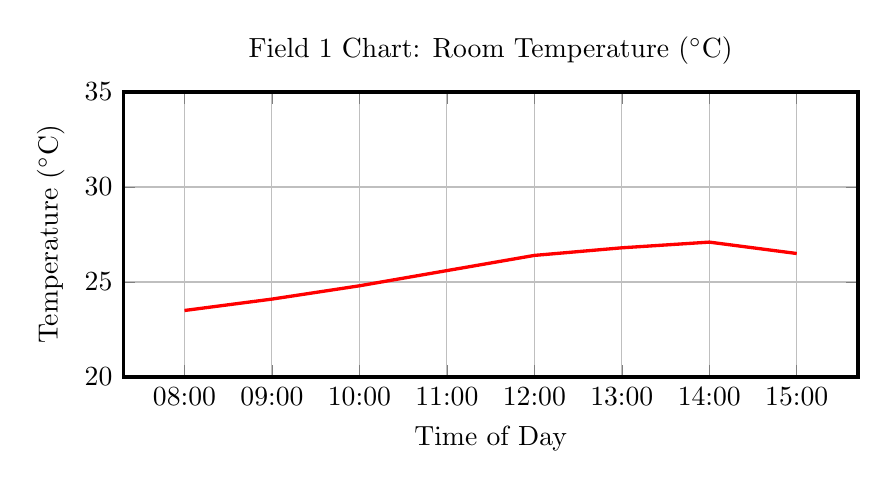
\begin{tikzpicture}
        \begin{axis}[
            width=0.9\textwidth,
            height=5.2cm,
            title={Field 1 Chart: Room Temperature ($^\circ$C)},
            xlabel={Time of Day},
            ylabel={Temperature ($^\circ$C)},
            grid=major,
            xtick={1,2,3,4,5,6,7,8},
            xticklabels={08:00, 09:00, 10:00, 11:00, 12:00, 13:00, 14:00, 15:00},
            ymin=20, ymax=35,
            line width=1.2pt,
            mark=*
        ]
        \addplot[color=red] coordinates {(1,23.5) (2,24.1) (3,24.8) (4,25.6) (5,26.4) (6,26.8) (7,27.1) (8,26.5)};
        \end{axis}
    \end{tikzpicture}
    
    \vspace{0.5cm}
    
    % ThingSpeak Graph 2: Voltage
    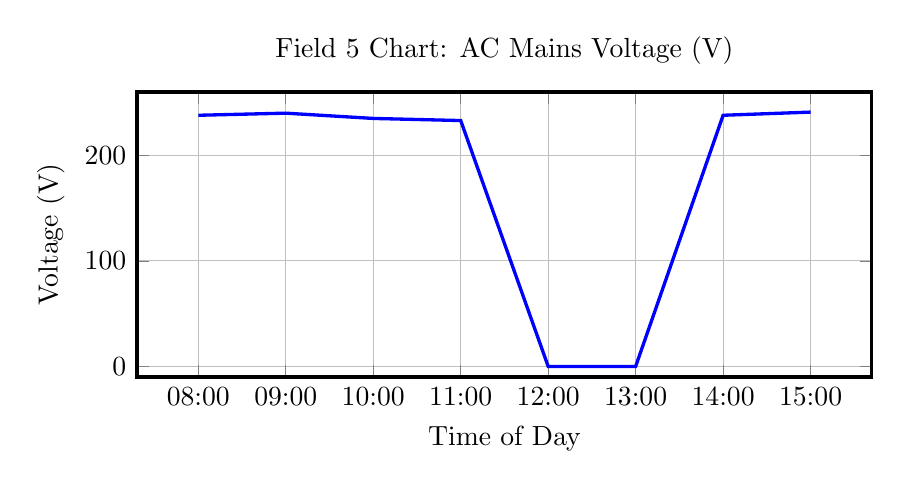
\begin{tikzpicture}
        \begin{axis}[
            width=0.9\textwidth,
            height=5.2cm,
            title={Field 5 Chart: AC Mains Voltage (V)},
            xlabel={Time of Day},
            ylabel={Voltage (V)},
            grid=major,
            xtick={1,2,3,4,5,6,7,8},
            xticklabels={08:00, 09:00, 10:00, 11:00, 12:00, 13:00, 14:00, 15:00},
            ymin=-10, ymax=260,
            line width=1.2pt,
            mark=square*
        ]
        \addplot[color=blue] coordinates {(1,238) (2,240) (3,235) (4,233) (5,0) (6,0) (7,238) (8,241)}; 
        % The drop to 0 represents the detected blackout at noon.
        \end{axis}
    \end{tikzpicture}
    \caption{ThingSpeak Web Dashboard data plots showing normal environmental temperature fluctuations alongside a detected power grid blackout event at 12:00.}
    \label{fig:thingspeak}
\end{figure}

\subsection{Multi-Server Cloud Ecosystem and Remote Control Architecture}
To prevent single-point-of-failure vulnerabilities and provide versatile interfaces for different operational roles, the system implements a multi-server architecture spanning Telegram, Discord, Google Colab, and Blynk:

\begin{enumerate}
    \item \textbf{Telegram Bot API (Interactive Alerts \& Control):} Utilizing the Telegram Bot API over HTTPS with TLS 1.2 encryption, the ESP32-CAM dispatches captured JPEG snapshots directly to authorized administrators via the \texttt{sendPhoto} endpoint upon intrusion detection. Administrators can also issue bidirectional chat commands such as \texttt{/status} (query live temperature, gas, and grid voltage), \texttt{/snap} (trigger an immediate on-demand surveillance capture), and \texttt{/relay\_on} or \texttt{/relay\_off} (remotely override the exhaust fan and safety actuators).
    
    \item \textbf{Discord Server Webhook Integration (Surveillance Log \& Alerts):} For centralized team monitoring, the system integrates Discord Incoming Webhooks. Security breaches and critical hazards trigger rich JSON embeds featuring color-coded status badges (e.g., Red for intrusion/gas leaks, Yellow for grid voltage fluctuations, and Green for nominal states). The ESP32-CAM uploads evidence snapshots directly into the surveillance channel and triggers emergency role pings (\texttt{@here} / \texttt{@admin}) during blackout or smoke conditions.
    
    \item \textbf{Google Colab Pipeline (Machine Learning \& Anomaly Analytics):} A continuous telemetry stream is ingested by a cloud-hosted Google Colab environment (interfaced via RESTful webhooks and Ngrok tunnel endpoints). A Python data science pipeline processes incoming time-series telemetry using Pandas and Scikit-learn. An unsupervised Isolation Forest algorithm flags anomalous power consumption spikes and voltage transients, while linear regression models forecast daily energy usage ($kWh$) and evaluate HVAC efficiency.
    
    \item \textbf{Blynk IoT Cloud Platform (Mobile Dashboard \& Virtual Pins):} For high-responsiveness handheld monitoring, the prototype synchronizes with the Blynk 2.0 Cloud. Hardware telemetry is bound to Virtual Pins: $V_0$ (Ambient Temperature), $V_1$ (Relative Humidity), $V_2$ (Gas Concentration in PPM), $V_3$ (Exhaust Fan Relay toggle), $V_4$ (Intrusion Alarm state), and $V_5$ (AC Mains Voltage). The native iOS/Android Blynk application provides live gauge meters, push notifications, and tactile toggle switches.
\end{enumerate}

\begin{table}[H]
\centering
\caption{Comparative Matrix of Multi-Server Integration Options}
\label{tab:servers_comparison}
\resizebox{\textwidth}{!}{%
\begin{tabular}{|l|l|c|l|p{5cm}|}
\hline
\textbf{Server / Platform} & \textbf{Protocol} & \textbf{Latency} & \textbf{Media Payload} & \textbf{Primary Operational Role} \\ \hline
Telegram Bot API & HTTPS / REST & $< 1.5$ s & JPEG Snapshots & Personal intrusion alerts \& chat command actuation \\ \hline
Discord Webhook & HTTPS / JSON & $< 1.0$ s & Embeds + Images & Collaborative team surveillance log \& incident feed \\ \hline
Google Colab & REST / HTTP POST & $\approx 2.5$ s & Tabular Telemetry & ML anomaly detection, regression \& power profiling \\ \hline
Blynk IoT Cloud & TCP / Blynk REST & $< 0.8$ s & Pin Values & Real-time mobile dashboard gauges \& relay switches \\ \hline
ThingSpeak & HTTP GET / POST & $15$ s & 8-Field Numerical & Long-term cloud trend logging \& public web charts \\ \hline
\end{tabular}%
}
\end{table}

\subsection{Universal Serial Device Output Examiner and 120+ Sensor Template Library}
To support universal serial interoperability across heterogeneous microcontrollers and sensor technologies, the system incorporates an intelligent \textbf{Universal Serial Output Examiner} backed by an extensive repository of over 120 sensor, actuator, and device templates. This architecture eliminates vendor lock-in by dynamically inspecting arbitrary serial data streams, classifying signal protocols, and matching telemetry signatures against known hardware models.

\begin{enumerate}
    \item \textbf{Heuristic Pattern Recognition Engine:} The serial examiner parses unformatted asynchronous UART streams, identifying transmission framing such as JSON objects, key-value comma-delimited strings (\texttt{TEMP:24.2,HUM:58.4}), raw 10-bit/12-bit ADC integer streams, GPS NMEA sentences, and cellular AT command responses. A multi-tier scoring algorithm correlates regex signatures, token names, and mathematical value domains to compute a percentage match confidence for candidate sensor models.
    
    \item \textbf{Comprehensive 120+ Sensor \& Actuator Classification:} The template library classifies devices across analog and digital paradigms, standardizing pinouts, operating voltages, calibration equations, and baud configurations across 10 functional domains:
    \begin{itemize}
        \item \textbf{Climate \& Temperature (16 Models):} Digital single-bus (DHT11, DHT22, AM2302), Dallas 1-Wire (DS18B20), I$^2$C/SPI environmental sensors (BME280, BMP280, BME680, SHT31, SHT40, AHT20, Si7021, MCP9808), linear analog sensors (LM35 10~mV/$^\circ$C, TMP36), analog resistance dividers (NTC 10K MF52 Steinhart-Hart), and platinum RTDs (PT100 with MAX31865).
        \item \textbf{Gas, Smoke \& Hazardous Fumes (18 Models):} Metal-oxide semiconductor modules (MQ-2 smoke, MQ-3 alcohol, MQ-4 methane, MQ-5 LPG, MQ-6 propane, MQ-7 CO cyclic, MQ-8 hydrogen, MQ-9 dual-gas, MQ-135 air quality, MQ-136 H$_2$S, MQ-137 ammonia, MQ-138 VOCs), multi-pixel digital sensors (SGP30, SGP40), optical NDIR detectors (Winsen MH-Z19B, Senseair S8, Sensirion SCD30), and laser dust sensors (Plantower PMS5003).
        \item \textbf{AC Power, Voltage \& Current (10 Models):} Active voltage transformers (ZMPT101B 0--250~V AC), Hall-effect current sensors (Allegro ACS712-05A/20A/30A), non-invasive split-core current transformers (SCT-013-000, SCT-013-030), and multi-function energy meters (Peacefair PZEM-004T v3.0 UART, PZEM-016 Modbus-RS485, HLW8032, and INA219 DC power).
        \item \textbf{Gas Valves, Actuators \& HVAC Controls (16 Models):} 12~V brass electromagnetic solenoid shutoff valves (2W-160-15), 3-wire motorized ball valves (DN15-CR02 with limit feedback), automatic pipe shutoff manipulator arms, Tuya Wi-Fi smart AC gateways, Midea split AC UART dongles (OSK-103 9600 baud), Mitsubishi CN105 heatpump serial adapters (2400 baud 8-E-1), Daikin S21 serial split AC bridges, Modbus RTU RS485 fan coil thermostats, 38~kHz infrared AC blasters, optocoupled relays (1-channel, 4-channel), solid-state relays (SSR-25DA zero-crossing), and 24~V motorized HVAC damper actuators (Belimo LM24A).
        \item \textbf{Motion, Radar \& Optical (26 Models):} Passive infrared detectors (HC-SR501, HC-SR505, AM312), Doppler microwave radar (RCWL-0516 3.18~GHz), 24~GHz human static presence mmWave radar (HLK-LD2410), ultrasonic distance rangers (HC-SR04, waterproof JSN-SR04T), Time-of-Flight laser sensors (VL53L0X, Benewake TFmini Plus), magnetic reed switches (MC-38), 6-axis IMUs (MPU-6050, ADXL345), ambient light sensors (GL5528 LDR, BH1750, TSL2561, TSL2591), pulse oximeters (MAX30102), and non-contact infrared thermopiles (MLX90614, AMG8833 Grid-EYE).
        \item \textbf{Liquid, Soil, Wireless \& Controllers (38 Models):} Capacitive soil moisture (HW-390 v1.2), submersible hydrostatic level transmitters (4--20~mA loop), YF-S201 Hall water flow meters, analog TDS and pH meters (E-201-C), BLE beacons (Xiaomi LYWSD03MMC, Inkbird IBS-TH2, RuuviTag B8), Shelly Plus H\&T Wi-Fi, Sonoff Zigbee, ESP-NOW radios, SIM800L cellular, SIM7600E-H 4G LTE, and target microcontroller boards (ESP32-CAM, Spark Core Particle STM32, Arduino Uno/Mega, and STM32 Blue Pill).
    \end{itemize}
    
    \item \textbf{Turnkey Multi-Sensor Firmware Generation:} Users can select any combination of catalog sensor profiles to instantly synthesize compile-ready Arduino C++ sketches. The generator provisions precise GPIO pin mapping, baud rate configuration, header inclusion, and structured JSON serial streaming compatible with Sanctuary OS and KyU Telemetry endpoints.
\end{enumerate}

\begin{table}[H]
\centering
\caption{Comparison of Primary Sensor Signal Categories and Operating Characteristics}
\label{tab:sensor_signal_matrix}
\resizebox{\textwidth}{!}{%
\begin{tabular}{|l|l|l|c|l|l|}
\hline
\textbf{Sensor Category} & \textbf{Typical Signal Type} & \textbf{Output Domain} & \textbf{Supply Voltage} & \textbf{Primary Models} & \textbf{Noise Immunity} \\ \hline
Analog ADC & Continuously Variable & 0 -- 3.3~V / 0 -- 5.0~V & 3.3~V / 5.0~V & LM35, ZMPT101B, MQ-2, LDR & Moderate (Requires Filtering) \\ \hline
Digital Single-Bus & Bidirectional 1-Wire & Asynchronous Pulse Width & 3.3~V -- 5.0~V & DHT11, DHT22, AM2302 & High (Parity / Checksum) \\ \hline
Dallas 1-Wire & 64-bit Addressable Bus & Digital Bit-Banging & 3.0~V -- 5.5~V & DS18B20 & High (CRC8 Verification) \\ \hline
I$^2$C Serial Bus & Synchronous 2-Wire & Serial Packets (SCL/SDA) & 1.8~V -- 3.3~V & BME280, SGP30, BH1750, MPU-6050 & Very High (Bus Protocol) \\ \hline
UART / RS485 & Asynchronous Serial & ASCII / Modbus RTU & 5.0~V / 12--24~V & PZEM-004T, MH-Z19B, PMS5003 & Excellent (Differential on RS485) \\ \hline
Actuator / Valve & Digital / PWM Switching & Coil State / Pulse Width & 5.0~V / 12--24~V & 12V Solenoid, Motorized Ball, Relay & Isolated (Optocoupler / Flyback) \\ \hline
Wireless BLE / RF & 2.4~GHz Radio Packets & Bluetooth Advertisements & 3.0~V (Battery) & LYWSD03MMC, RuuviTag, ESP-NOW & Maximum (No Galvanic Lines) \\ \hline
\end{tabular}%
}
\end{table}

\subsection{Multi-Premise Architectural Models and Interactive Drag-and-Drop Area Layout System}
To accommodate diverse industrial, enterprise, and residential deployments, the platform implements a modular \textbf{Multi-Premise Architectural Engine} and an interactive zero-dependency HTML5 \textbf{Drag-and-Drop Facility Layout Canvas}. This architecture abstracts physical locations into secure spatial zones, providing purpose-built telemetry displays, dedicated actuator controls, and automatic sensor ingestion directly from serial streams.

\begin{enumerate}
    \item \textbf{Comprehensive Multi-Premise Archetype Engine:} The system provides six turnkey facility models with pre-configured spatial zones, operational clearance levels, and domain-specific sensor payloads:
    \begin{itemize}
        \item \textbf{Smart Residential Home:} Focuses on ambient indoor comfort, fire safety, and energy efficiency. Pre-configured zones include the \textit{Living Room} (DHT22 climate, MQ-2 smoke, Tuya AC thermostat), \textit{Kitchen \& Pantry} (MQ-4 methane, optical flame detector, 12~V emergency solenoid shutoff valve), \textit{Master Suite} (BMP280 barometric pressure, BH1750 ambient lux), \textit{Front Entrance \& Porch} (RCWL-0516 microwave radar, MC-38 magnetic door reed switch, piezo siren), and \textit{Electrical Utility Hub} (ZMPT101B AC voltage transformer, ACS712 current sensor, mains relay).
        
        \item \textbf{Telecom Base Station \& Perimeter Fence:} Engineered for mission-critical cellular towers and remote microwave repeater sites subject to physical tampering and extreme weather. Key operational zones comprise:
        \begin{itemize}
            \item \textit{Perimeter Security Fence:} Features HB100 X-band Doppler microwave radar barriers, SW-420 fence vibration sensors, infrared laser tripwires, and high-intensity 500~W strobe floodlight relays for immediate intrusion deterrence.
            \item \textit{BTS Equipment Shelter:} Houses rack-mounted transceivers, monitored by BME280 precision climate transducers, smoke detectors, and redundant Computer Room Air Conditioning (CRAC) unit controllers.
            \item \textit{Battery \& UPS Room:} Continuously monitors 48~V DC backup battery strings via INA219 current/power monitors, PZEM-016 DC energy meters, and MQ-8 hydrogen gas detectors to avert explosive outgassing during thermal runaway charging.
            \item \textit{Tower Mast \& Antenna Array:} Instruments structural mast deflection using MPU-6050 6-axis accelerometers, cups-anemometer wind velocity meters, and aviation obstruction beacon monitoring circuits.
            \item \textit{Diesel Generator \& Fuel Depot:} Tracks reserve diesel levels via TL-136 submersible hydrostatic pressure transducers (4--20~mA loop), engine block temperature probes (DS18B20), and automated backup genset starter interlocks.
        \end{itemize}
        
        \item \textbf{Hospital \& Medical Campus:} Tailored for high-dependency clinical environments, sterile surgical suites, and biological cryo-chains. Zones encompass the \textit{Intensive Care Unit (ICU)} (AD8232 dynamic electrocardiogram ECG telemetry, MAX30102 pulse oximetry, MLX90614 non-contact infrared patient thermopiles), \textit{Vaccine \& Blood Cryo-Vault} (ultra-low $-80^\circ$C PT100 RTDs, audible cold-chain breach alarms), \textit{Surgical Operating Theater} (laminar positive differential air pressure transducers, NDIR CO$_2$, trace halogenated anesthetic gas detectors), \textit{Negative Pressure Isolation Ward} (airborne pathogen containment pressure monitoring, UV-C germicidal sterilization relays), and the \textit{Medical Oxygen Manifold} (cryogenic O$_2$ high-pressure transducers, ultrasonic mass flow meters, and emergency shutoff valves).
        
        \item \textbf{Industrial Chemical \& Manufacturing Plant:} Provisions heavy factory automation and hazmat safety. Encompasses the \textit{Chemical Synthesis Bay} (corrosive MQ-136 H$_2$S and MQ-137 ammonia monitors, motorized PTFE acid ball valves), \textit{High-Pressure Steam Boiler Room} (Wika industrial pressure transducers, PT100 boiler core probes, optical ultraviolet/infrared burner flame scanners), \textit{Automated Conveyor Line} (Omron inductive proximity part counters, bearing vibration sensors, hardwired Emergency Stop E-stop interlocks), and the \textit{Hazardous Solvent Depot} (Figaro TGS2610 explosive vapor detectors, deluge foam suppression relays).
        
        \item \textbf{Smart Agriculture \& Commercial Greenhouse:} Designed for precision agronomy and hydroponic automation. Zones include the \textit{Hydroponics Nutrient Bay} (analog pH glass probes, electrical conductivity / TDS sensors, Hall-effect recirculation flow meters), \textit{Greenhouse Canopy Climate} (Sensirion SCD30 photoacoustic CO$_2$, Apogee SQ-500 Photosynthetically Active Radiation PAR lux sensors, high-pressure misting fogger relays), and the \textit{Precision Drip Field} (multi-depth capacitive soil moisture probes, soil temperature probes, and Hunter 24~V AC solenoid irrigation valves).
        
        \item \textbf{Enterprise Data Center:} Safeguards high-density server racks through \textit{Cold Aisle Containment} (inlet temperature sensors, differential pressure gauges, electronically commutated variable-frequency fan speed controls), \textit{Hot Aisle Heat Exhaust} (exhaust damper servo actuators), \textit{Main Power Distribution (PDU)} (PZEM-016 3-phase metering, 500~A Hall-effect current transformers, remote substation breaker trip relays), and \textit{Subfloor Environmental Monitoring} (conductive sensing rope for fluid leak detection, sump pump evacuation).
    \end{itemize}
    
    \item \textbf{Interactive Drag-and-Drop Facility Layout Canvas:} Built using native HTML5 drag-and-drop APIs without external UI dependencies. Operators can visually rearrange facility zones, drag sensor chips between zones to reallocate physical coverage, and drag new devices directly from a searchable 124+ sensor template palette into any room. A custom zone creation modal allows operators to provision new spatial areas with distinctive iconography, operational purpose notes, and multi-tier security clearance levels (\textit{Public, General, Safety Critical, Restricted, Hazardous, Sterile, Biohazard Level 3}).
    
    \item \textbf{Rich Visual Designs with Dedicated Interactive Controls:} Each sensor widget features custom animated visuals, calibrated metric scales, and operational hardware control trays:
    \begin{itemize}
        \item \textit{Climate Thermostats:} Display ambient vs. setpoint temperatures, a dual-direction slider bar, and mode selector buttons (\textit{Cool, Heat, Fan, Auto}).
        \item \textit{Toxic \& Flammable Gas Gauges:} Incorporate animated circular SVG PPM gauges with color-coded safety thresholds, an audible siren test button, and a one-touch emergency gas solenoid trip interlock.
        \item \textit{AC/DC Power Monitors:} Feature multi-parameter voltage, current, active power, and cumulative energy readouts paired with a simulated circuit breaker trip and reset switch.
        \item \textit{Motorized Valves \& Solenoids:} Include animated fluid piping graphics with active flow particles, Open/Close toggle states, and 12~V 100~ms pulse triggering for pulse-latching valves.
        \item \textit{Hydrostatic Liquid Columns:} Display animated tank fluid columns with dynamic wave surfaces, volumetric capacity percentages, and auto-fill pump toggles.
        \item \textit{Perimeter Radar Sentinels:} Feature a real-time revolving radar beam sweep animation, detection sensitivity range controls, and perimeter strobe floodlight triggers.
        \item \textit{Biometric Vital Signs:} Render a continuous SVG electrocardiogram (ECG) pulse waveform, live SpO$_2$ and heart rate metrics, and a direct nurse call alert station trigger.
    \end{itemize}
    
    \item \textbf{Autonomous Serial Telemetry Detection \& Sensor Ingestion:} When serial devices stream data via Web Serial, USB COM ports, or wireless bridges, the heuristic examination engine matches the incoming packet signature against the 124+ catalog profiles. If an unmapped sensor signature is detected with confidence $\ge 60\%$, the system automatically instantiates a rich sensor widget in the appropriate facility zone without requiring manual configuration, broadcasting an operator toast notification and logging the hardware pairing.
\end{enumerate}

\subsection{Cost Analysis and Bill of Materials}
A critical deliverable was the formulation of the Bill of Materials (BOM) for a scaled deployment of 100 units. The estimation assumes bulk purchasing discounts. 

\begin{table}[H]
\centering
\caption{Estimated Bill of Materials (BOM) and Cost Analysis for 100-Unit Deployment (Deliverable 4)}
\label{tab:bom}
\resizebox{0.95\textwidth}{!}{%
\begin{tabular}{|l|c|c|c|}
\hline
\textbf{Component} & \textbf{Unit Price (USD)} & \textbf{Qty / Unit} & \textbf{Cost (100 Units)} \\ \hline
ESP32-CAM Module & \$ 5.50 & 1 & \$ 550.00 \\ \hline
SIM800L GSM Module & \$ 3.50 & 1 & \$ 350.00 \\ \hline
Power Sensors (Voltage/Current) & \$ 4.00 & 1 set & \$ 400.00 \\ \hline
Environment \& Safety Sensors & \$ 7.00 & 1 set & \$ 700.00 \\ \hline
Peripherals (Relay, Buzzer, Reed) & \$ 3.00 & 1 set & \$ 300.00 \\ \hline
Fabrication (PCB, Enclosure, Power) & \$ 10.00 & 1 set & \$ 1,000.00 \\ \hline
\textbf{Total Estimated BOM Cost} & \textbf{\$ 33.00} & \textbf{-} & \textbf{\$ 3,300.00} \\ \hline
\end{tabular}%
}
\end{table}

\section{Conclusion}
The Level 2 Smart Room Monitoring System was successfully designed and tested, meeting all project requirements. The transition to the ESP32-CAM enabled critical visual verification of intrusions, while the SIM800L ensured that alerts reached the administrator even during internet outages. The inclusion of power monitoring sensors provided valuable data regarding AC grid stability. By integrating a versatile multi-server cloud ecosystem spanning Telegram, Discord, Google Colab, Blynk, and ThingSpeak, the project delivered a robust, fault-tolerant IoT solution suitable for real-world deployment in environments subject to power and network instability.

\end{document}
